\lhead[\thepage]{CAPÍTULO \thechapter. ANÁLISIS}
\chead[]{}
\rhead[WepSIM: Simulador de procesador elemental con unidad de control microprogramada\leftmark]{\thepage}
\renewcommand{\headrulewidth}{0.5pt}

\lfoot[]{}
\cfoot[]{}
\rfoot[]{}
\renewcommand{\footrulewidth}{0pt}

%% This is an example first chapter.  You should put chapter/appendix that you
%% write into a separate file, and add a line \include{yourfilename} to
%% main.tex, where `yourfilename.tex' is the name of the chapter/appendix file.
%% You can process specific files by typing their names in at the 
%% \files=
%% prompt when you run the file main.tex through LaTeX.
\chapter{Análisis}
\label{ch:analysis}
\markboth{}{ANALYSIS}

El objetivo principal de este capitulo, es describir el proyecto mediante la obtención y especificación de los requisitos del simulador, que puede proporcionar información suficiente para un análisis detallado que, por lo tanto, puede servir para continuar diseñando e implementando (Capítulos \ref{ch:design}, \textit{\nameref{ch:design}}; and \ref{ch:implementation_and_deployment}, \textit{\nameref{ch:implementation_and_deployment}}) un software que cumpla con esos requisitos. 

Con el fin de obtener los requisitos del sistema, el tutor ha desempeñado el papel del cliente en diferentes reuniones, mientras que el alumno ha desempeñado los roles de analista, diseñador, programador y probador.

La sección \ref{sec:project_description} resume brevemente la descripción del proyecto. La sección \ref{sec:solution_selection} discute la solución elegida y la compara con las alternativas consideradas. La sección \ref{sec:requirements} especifica los requisitos del sistema, empezando con los requisitos de usuario y finalizando con los requisitos funcionales y no-funcionales. Finalmente, la sección \ref{sec:regulatory_framework} indica el conjunto de leyes y regulaciones para la gestión del software.  

\section{Descripción del proyecto}
\label{sec:project_description}

El objetivo de este proyecto es construir una herramienta que permita simular con realismo el comportamiento de un procesador basado en la arquitectura indicada por el el tutor del proyecto, de forma que sirva como única herramienta para los alumnos a lo largo de la asignatura Estructura de Computadores.

\begin{figure}[htbp]
 	\centering
 	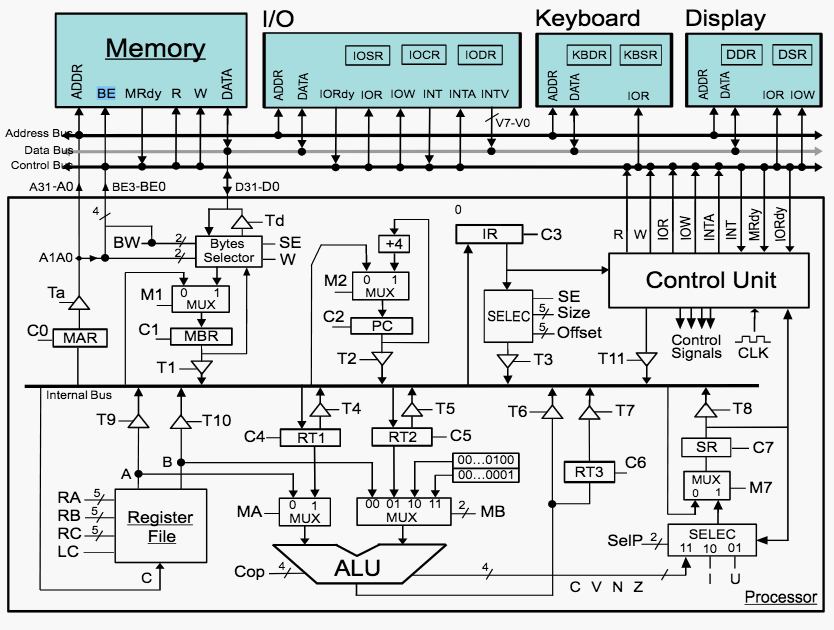
\includegraphics[width=12cm]{figures/cpu}
 	\caption{Arquitectura CPU WepSIM .}
	\label{fig:wepsimCPU_figure}
\end{figure}

\begin{figure}[htbp]
 	\centering
 	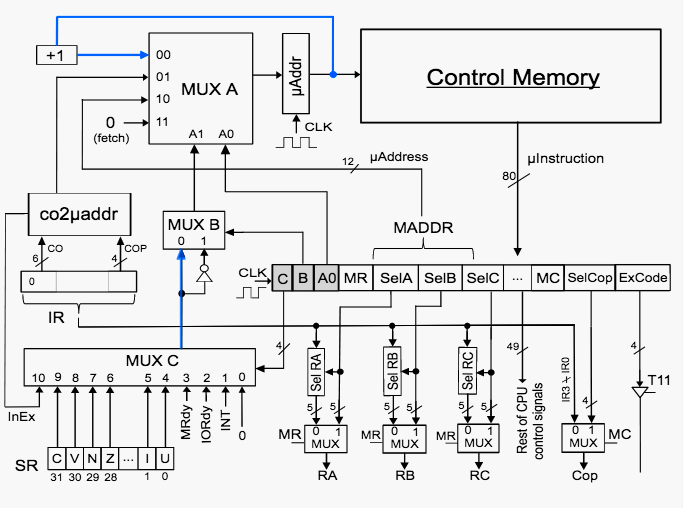
\includegraphics[width=12cm]{figures/controlUnit}
 	\caption{Arquitectura unidad de control WepSIM.}
	\label{fig:wepsimCU_figure}
\end{figure}

Los simuladores actuales para la enseñanza de Estructura de Computadores, están focalizados a una función concreta, como puede ser la simulación de cachés, la simulación de código ensamblador o la simulación de microcódigo entre otros, pero a la hora de unificar todas estas funcionalidades en una única herramienta, existe un vacío que genera una pérdida de tiempo en el aprendizaje de cada herramienta y la no posibilidad de ver una simulación completa.

El reto al que se enfrente cualquier simulador educativo es el de ser capaz de simular fielmente el funcionamiento de un dispositivo permitiendo al estudiante poder observar con el mayor detalle posible el comportamiento éste.

El sistema que se propone debe ser capaz de simular con realismo el comportamiento del procesador, permitiendo la definición del juego de instrucciones a utilizar para el posterior desarrollo de código ensamblador y su ejecución en el simulador con un alto nivel de detalle en cada uno de los ciclos de ejecución,.De esta forma, los estudiantes podrán comprender fácilmente los contenidos teóricos expuestos en la asignatura y serán capaces de realizar todas las prácticas en una misma herramienta, pudiendo ver de forma incremental el desarrollo de software de bajo nivel sobre un procesador elemental.


\section{Solución elegida}
\label{sec:solution_selection}

Para que los profesores de la asignatura Estructura de Computadores puedan hacer uso de una herramienta que sirva de ayuda para la explicación de los conceptos teóricos de la asignatura, y los alumnos puedan utilizarla para comprender estos conceptos y realizar posteriormente las prácticas de la asignatura, se propone el diseño e implementación de una herramienta web que simule con realismo en funcionamiento de un procesador elemental con unidad de control microprogramable.

Este simulador, será desarrollado como una herramienta web debido a la portabilidad que proporciona, ya que podrá ser ejecutado sobre un gran número de diferentes dispositivos independientemente del sistema operativo que utilice, puesto que únicamente necesita un navegador web para su correcto funcionamiento. De esta forma, los profesores y alumnos podrán hacer uso de la herramienta sin depender de su instalación en el dispositivo a utilizar, incluso pudiendo los alumnos realizar las prácticas sobre dispositivos móviles.

Además, se ha elegido que el proyecto sea desarrollado en el lenguaje de programación Javascript, debido a las facilidades que proporciona para la posterior generación automática mediante el framework de desarrollo Apache Cordova de aplicaciones móviles para las plataformas móviles Android e iOS y de aplicaciones para el sistema operativo Windows. De esta forma, con un único desarrollo, se obtiene un amplio abanico de plataformas sobre las que poder utilizar la herramienta sin tener dependencia de conexión a internet.

Por tanto, la solución elegida es capaz de unificar en una misma herramienta todas las funcionalidades requeridas para la enseñanza de Estructura de computadores con un alto nivel de detalle, con alta disponibilidad al facilitarse su como una herramienta web, y con una gran portabilidad puesto que podrá ser ejecutada sobre un gran número de diversos dispositivos.


\section{Requisitos}
\label{sec:requirements}

Esta sección proporciona una descripción detallada de los requisitos de la aplicación. Para la tarea de la especificación de requisitos, se han seguido las prácticas recomendadas por IEEE \cite{ieee1998}. De acuerdo con estas prácticas, una buena especificación debe abordar la funcionalidad del software, los problemas de rendimiento, las interfaces externas, otras características no funcionales y las limitaciones de diseño o implementación.
Además, la especificación de los requisitos debe ser:

\begin{itemize}

\item \textbf{Completa:} el documento refleja todos los requisitos de software importantes.

\item \textbf{Consistente:} los requisitos no deben generar conflictos entre sí.

\item \textbf{Correcta:} cada requisito debe ser cumplido por el software según las necesidades del usuario.

% every requirement is one that the software shall meet according to the user needs.

\item \textbf{Modificable:} la estructura de la especificación permite cambios en los requisitos de una manera simple, completa y consistente.

\item \textbf{Clasificación basada en la importancia y la estabilidad:} cada requisito debe indicar su importancia y su estabilidad.

\item \textbf{Trazable:} el origen de cada requisito es claro y se puede hacer referencia fácilmente en otras etapas.

\item \textbf{Inequívoco:} cada requisito tiene una sola interpretación.

\item \textbf{Verificable:} Cada requisito debe ser verificable, es decir, existe algún proceso para verificar que el software cumple con cada requisito.

\end{itemize}

A partir de los requisitos de los usuarios, que constituyen una referencia informal al comportamiento del producto que el cliente espera, derivamos los requisitos de software (en este caso, requisitos funcionales y no funcionales) que guiaron el proceso de diseño con información específica sobre la funcionalidad del sistema y otras características. Los requisitos recuperados se estructuraron de acuerdo con el siguiente esquema:

%Starting from the user requirements, which constitute an informal reference to the product p%erformance that the client expects, we derived the software requirements (in this case, functional r%equirements and non-functional requirements) that guided the design process with specific %nformation on the functionality of the system and other characteristics. The retrieved requirements %were structured according with the following schema:

\begin{itemize}
\item[1.] \textbf{Requisitos de Usuario} 
	\begin{itemize}
		\item[(a)] \textbf{Capacidad:} el requisito describe la funcionalidad esperada del sistema como en casos de uso.
		\item[(b)] \textbf{Restricción:} el requisito especifica las restricciones o condiciones que el sistema debe cumplir.
	\end{itemize}	
\end{itemize}

\begin{itemize}
\item[2.] \textbf{Requisitos de Software}
	\begin{itemize}
	\item[(a)] 	\textbf{Funcionales}
		\begin{itemize}
		\item[i.] 	\textbf{Funcional:} el requisito describe la funcionalidad básica y el propósito del sistema mientras se minimiza la ambigüedad.
		\item[ii.] 	\textbf{Inverso:} el requisito limita la funcionalidad de la aplicación para aclarar su alcance.
		\end{itemize}

	\item[(b)] 	\textbf{No-Funcionales}
		\begin{itemize}
		\item[i.] 	\textbf{Rendimiento:} el requisito se relaciona con el rendimiento mínimo requerido del sistema resultante.
		\item[ii.] 	\textbf{Interfaz:} el requisito está relacionado con la interfaz de usuario de la aplicación.
		\item[iii.] 	\textbf{Escalabilidad:} el requisito está relacionado con la capacidad del sistema para adaptarse a cargas de trabajo cada vez mayores.
		\item[iv.] 	\textbf{Plataforma:} el requisito especifica las plataformas subyacentes de software y hardware en las que funcionará el sistema.
		\end{itemize}			
	\end{itemize}
\end{itemize}

Table \ref{tab:requirements_template} proporciona la plantilla utilizada para la especificación de requisitos. Tenga en cuenta que para los requisitos del usuario, el formato de identificación será UR-XYY, donde X indica el subtipo de requisito: requisitos de capacidad (C) o restricciones (R). YY corresponde al número de requisito en su subcategoría. Para los requisitos de software, se utilizará el formato de identificación SR-X-YZZ, donde X indica si es un requisito funcional (F) o no funcional (NF), e Y representa su subcategoría: funcional (F), inversa (I) ), Rendimiento (P), interfaz (UI), escalabilidad (S) o plataforma (PL). ZZ corresponde al número de requisito en su subcategoría.

\begin{center}
\begin{table*}[htbp]
\centering
\begin{tabular}{@{}p{2.5cm} p{9cm}@{}} 
\toprule
\textbf{ID} 				& Requisito ID. \\
\midrule
\textbf{Nombre} 			& Nombre del requisito. \\
\midrule
\textbf{Tipo} 			& Indica la categoría en la que se colocaría el requisito de acuerdo con el esquema descrito anteriormente. \\
\midrule
\textbf{Origen} 			& Constituye la fuente del requisito. Puede ser el usuario, otro requisito u otros actores involucrados en el proyecto. \\
\midrule
\textbf{Prioridad}		& Indica la prioridad del requisito según su importancia. Un requisito puede ser identificado como \textit{esencial}, \textit{condicional} or \textit{opcional}. \\
\midrule
\textbf{Estabilidad} 		& Indica la variabilidad del requisito a través del proceso de desarrollo, definido como \textit{estable} or \textit{inestable}. \\
\midrule
\textbf{Descripción} 	& Explicación detallada del requisito. \\
\bottomrule
\end{tabular}
\caption{Plantilla para la especificación de requisitos.}
\label{tab:requirements_template}
\end{table*}
\end{center}

\subsection{Requisitos de Usuario}

Esta subsección especifica los requisitos de usuario.

\begin{center}
\begin{table*}[htbp]
\centering
\begin{tabular}{@{}p{2.5cm} p{9cm}@{}} 
\toprule
\textbf{ID} 				& UR-C01 \\
\midrule
\textbf{Nombre} 			& Simulación del modelo hardware propuesto\\
\midrule
\textbf{Tipo} 			& Capacidad \\
\midrule
\textbf{Origen} 			& Usuario \\
\midrule
\textbf{Prioridad}		& Esencial \\
\midrule
\textbf{Estabilidad} 		& Estable \\
\midrule
\textbf{Descripción} 	& La herramienta debe realizar la simulación de códigos ensamblador sobre la arquitectura definida. \\
\bottomrule
\end{tabular}
\caption{Requisito de usuario UR-C01.}
\label{tab:urc01}
\end{table*}
\end{center}

\begin{center}
\begin{table*}[htbp]
\centering
\begin{tabular}{@{}p{2.5cm} p{9cm}@{}} 
\toprule
\textbf{ID} 				& UR-C02 \\
\midrule
\textbf{Nombre} 			& Definición de juego de instrucciones del simulador \\
\midrule
\textbf{Tipo} 			& Capacidad \\
\midrule
\textbf{Origen} 			& Usuario \\
\midrule
\textbf{Prioridad}		& Esencial \\
\midrule
\textbf{Estabilidad} 		& Estable \\
\midrule
\textbf{Descripción} 	& La herramienta debe permitir la definición del juego de instrucciones a utilizar por el usuario. \\
\bottomrule
\end{tabular}
\caption{Requisito de usuario UR-C02.}
\label{tab:urc02}
\end{table*}
\end{center}

\begin{center}
\begin{table*}[htbp]
\centering
\begin{tabular}{@{}p{2.5cm} p{9cm}@{}} 
\toprule
\textbf{ID} 				& UR-C03 \\
\midrule
\textbf{Nombre} 			& Definición de código ensamblador a simular \\
\midrule
\textbf{Tipo} 			& Capacidad \\
\midrule
\textbf{Origen} 			& Usuario \\
\midrule
\textbf{Prioridad}		& Esencial \\
\midrule
\textbf{Estabilidad} 		& Estable \\
\midrule
\textbf{Descripción} 	& La herramienta debe permitir la definición del código ensamblador a utilizar en la simulación por el usuario. \\
\bottomrule
\end{tabular}
\caption{Requisito de usuario UR-C03.}
\label{tab:urc03}
\end{table*}
\end{center}

\begin{center}
\begin{table*}[htbp]
\centering
\begin{tabular}{@{}p{2.5cm} p{9cm}@{}} 
\toprule
\textbf{ID} 				& UR-C04 \\
\midrule
\textbf{Nombre} 			& Información del estado del procesador durante la simulación \\
\midrule
\textbf{Tipo} 			& Capacidad \\
\midrule
\textbf{Origen} 			& Usuario \\
\midrule
\textbf{Prioridad}		& Esencial \\
\midrule
\textbf{Estabilidad} 		& Estable \\
\midrule
\textbf{Descripción} 	& La herramienta debe mostrar el estado actual de procesador durante las simulaciones. \\
\bottomrule
\end{tabular}
\caption{Requisito de usuario UR-C04.}
\label{tab:urc04}
\end{table*}
\end{center}

\begin{center}
\begin{table*}[htbp]
\centering
\begin{tabular}{@{}p{2.5cm} p{9cm}@{}} 
\toprule
\textbf{ID} 				& UR-C05 \\
\midrule
\textbf{Nombre} 			& Configuración de las simulaciones \\
\midrule
\textbf{Tipo} 			& Capacidad \\
\midrule
\textbf{Origen} 			& Usuario \\
\midrule
\textbf{Prioridad}		& Esencial \\
\midrule
\textbf{Estabilidad} 		& Estable \\
\midrule
\textbf{Descripción} 	& La herramienta debe permitir la configuración de las simulaciones. \\
\bottomrule
\end{tabular}
\caption{Requisito de usuario UR-C05.}
\label{tab:urc05}
\end{table*}
\end{center}

\begin{center}
\begin{table*}[htbp]
\centering
\begin{tabular}{@{}p{2.5cm} p{9cm}@{}} 
\toprule
\textbf{ID} 				& UR-C06 \\
\midrule
\textbf{Nombre} 			& Compilación del código ensamblador según juego de instrucciones \\
\midrule
\textbf{Tipo} 			& Capacidad \\
\midrule
\textbf{Origen} 			& Usuario \\
\midrule
\textbf{Prioridad}		& Esencial \\
\midrule
\textbf{Estabilidad} 		& Estable \\
\midrule
\textbf{Descripción} 	& La herramienta debe realizar la compilación del código ensamblador dependiendo del juego de instrucciones definido previamente. \\
\bottomrule
\end{tabular}
\caption{Requisito de usuario UR-C06.}
\label{tab:urc06}
\end{table*}
\end{center}

\begin{center}
\begin{table*}[htbp]
\centering
\begin{tabular}{@{}p{2.5cm} p{9cm}@{}} 
\toprule
\textbf{ID} 				& UR-R01 \\
\midrule
\textbf{Nombre} 			& Arquitectura del simulador \\
\midrule
\textbf{Tipo} 			& Restricción \\
\midrule
\textbf{Origen} 			& Usuario \\
\midrule
\textbf{Prioridad}		& Esencial \\
\midrule
\textbf{Estabilidad} 		& Estable \\
\midrule
\textbf{Descripción} 	& La arquitectura del simulador debe ser la especificada por el tutor. \\
\bottomrule
\end{tabular}
\caption{Requisito de usuario UR-R01.}
\label{tab:urr01}
\end{table*}
\end{center}

\begin{center}
\begin{table*}[htbp]
\centering
\begin{tabular}{@{}p{2.5cm} p{9cm}@{}} 
\toprule
\textbf{ID} 				& UR-R02 \\
\midrule
\textbf{Nombre} 			& Juegos de instrucciones para el modelo hardware propuesto \\
\midrule
\textbf{Tipo} 			& Restricción \\
\midrule
\textbf{Origen} 			& Usuario \\
\midrule
\textbf{Prioridad}		& Esencial \\
\midrule
\textbf{Estabilidad} 		& Estable \\
\midrule
\textbf{Descripción} 	& Los juegos de instrucciones deben definirse según la arquitectura del simulador. \\
\bottomrule
\end{tabular}
\caption{Requisito de usuario UR-R02.}
\label{tab:urr02}
\end{table*}
\end{center}

\begin{center}
\begin{table*}[htbp]
\centering
\begin{tabular}{@{}p{2.5cm} p{9cm}@{}} 
\toprule
\textbf{ID} 				& UR-R03 \\
\midrule
\textbf{Nombre} 			& Formato del juego de instrucciones \\
\midrule
\textbf{Tipo} 			& Restricción \\
\midrule
\textbf{Origen} 			& Usuario \\
\midrule
\textbf{Prioridad}		& Esencial \\
\midrule
\textbf{Estabilidad} 		& Estable \\
\midrule
\textbf{Descripción} 	& El formato del juego de instrucciones debe seguir el formato indicado por el tutor. \\
\bottomrule
\end{tabular}
\caption{Requisito de usuario UR-R03.}
\label{tab:urr03}
\end{table*}
\end{center}

\begin{center}
\begin{table*}[htbp]
\centering
\begin{tabular}{@{}p{2.5cm} p{9cm}@{}} 
\toprule
\textbf{ID} 				& UR-R04 \\
\midrule
\textbf{Nombre} 			& Formato del código ensamblador \\
\midrule
\textbf{Tipo} 			& Restricción \\
\midrule
\textbf{Origen} 			& Usuario \\
\midrule
\textbf{Prioridad}		& Esencial \\
\midrule
\textbf{Estabilidad} 		& Estable \\
\midrule
\textbf{Descripción} 	& El formato del código ensamblador debe seguir el formato del juego de instrucciones definido previamente. \\
\bottomrule
\end{tabular}
\caption{Requisito de usuario UR-R04.}
\label{tab:urr04}
\end{table*}
\end{center}

\begin{center}
\begin{table*}[htbp]
\centering
\begin{tabular}{@{}p{2.5cm} p{9cm}@{}} 
\toprule
\textbf{ID} 				& UR-R05 \\
\midrule
\textbf{Nombre} 			& Simulador como herramienta web \\
\midrule
\textbf{Tipo} 			& Restricción \\
\midrule
\textbf{Origen} 			& Usuario \\
\midrule
\textbf{Prioridad}		& Esencial \\
\midrule
\textbf{Estabilidad} 		& Estable \\
\midrule
\textbf{Descripción} 	& El simulador debe estar diseñado e implementado para su uso como herramienta web. \\
\bottomrule
\end{tabular}
\caption{Requisito de usuario UR-R05.}
\label{tab:urr05}
\end{table*}
\end{center}

\begin{center}
\begin{table*}[htbp]
\centering
\begin{tabular}{@{}p{2.5cm} p{9cm}@{}} 
\toprule
\textbf{ID} 				& UR-R06 \\
\midrule
\textbf{Nombre} 			& Entorno de ejecución del simulador \\
\midrule
\textbf{Tipo} 			& Restricción \\
\midrule
\textbf{Origen} 			& Usuario \\
\midrule
\textbf{Prioridad}		& Esencial \\
\midrule
\textbf{Estabilidad} 		& Estable \\
\midrule
\textbf{Descripción} 	& El simulador debe poder ser ejecutado en los principales navegadores web del mercado. \\
\bottomrule
\end{tabular}
\caption{Requisito de usuario UR-R06.}
\label{tab:urr06}
\end{table*}
\end{center}


\iffalse

\begin{center}
\begin{table*}[htbp]
\centering
\begin{tabular}{@{}p{2.5cm} p{9cm}@{}} 
\toprule
\textbf{ID} 				& UR-C00 \\
\midrule
\textbf{Nombre} 			& a \\
\midrule
\textbf{Tipo} 			& a \\
\midrule
\textbf{Origen} 			& a \\
\midrule
\textbf{Prioridad}		& a \\
\midrule
\textbf{Estabilidad} 		& a \\
\midrule
\textbf{Descripción} 	& a \\
\bottomrule
\end{tabular}
\caption{Requisito de usuario UR-C00.}
\label{tab:urc00}
\end{table*}
\end{center}


%\begin{center}
%\begin{table*}[htbp]
%\centering
%\begin{tabular}{@{}p{2.5cm} p{9cm}@{}} 
%\toprule
%\textbf{ID} 				& UR-C01\\
%\midrule
%\textbf{Name} 			& BOINC projects simulation \\
%\midrule
%\textbf{Type} 			& Capacity \\
%\midrule
%\textbf{Origin} 			& User \\
%\midrule
%\textbf{Priority}		& Essential \\
%\midrule
%\textbf{Stability} 		& Stable \\
%\midrule
%\textbf{Description} 	& The application shall simulate real BOINC projects. \\
%\bottomrule
%\end{tabular}
%\caption{User requirement UR-C01.}
%\label{tab:urc01}
%\end{table*}
%\end{center}

\begin{center}
\begin{table*}[htbp]
\centering
\begin{tabular}{@{}p{2.5cm} p{9cm}@{}} 
\toprule
\textbf{ID} 				& UR-C02\\
\midrule
\textbf{Name} 			& Client \gls{scheduling} \\
\midrule
\textbf{Type} 			& Capacity \\
\midrule
\textbf{Origin} 			& User \\
\midrule
\textbf{Priority}		& Essential \\
\midrule
\textbf{Stability} 		& Stable \\
\midrule
\textbf{Description} 	& The client scheduler of the simulator shall follow the actual BOINC client \gls{scheduling}. \\
\bottomrule
\end{tabular}
\caption{User requirement UR-C02.}
\label{tab:urc02}
\end{table*}
\end{center}

\begin{center}
\begin{table*}[htbp]
\centering
\begin{tabular}{@{}p{2.5cm} p{9cm}@{}} 
\toprule
\textbf{ID} 				& UR-C03\\
\midrule
\textbf{Name} 			& Simulation components \\
\midrule
\textbf{Type} 			& Capacity \\
\midrule
\textbf{Origin} 			& User \\
\midrule
\textbf{Priority}		& Essential \\
\midrule
\textbf{Stability} 		& Stable \\
\midrule
\textbf{Description} 	& The simulations shall cover all the elements present in the BOINC infrastructure. \\
\bottomrule
\end{tabular}
\caption{User requirement UR-C03.}
\label{tab:urc03}
\end{table*}
\end{center}

\begin{center}
\begin{table*}[htbp]
\centering
\begin{tabular}{@{}p{2.5cm} p{9cm}@{}} 
\toprule
\textbf{ID} 				& UR-R01\\
\midrule
\textbf{Name} 			& Linux as underlying OS \\
\midrule
\textbf{Type} 			& Restriction \\
\midrule
\textbf{Origin} 			& User \\
\midrule
\textbf{Priority}		& Essential \\
\midrule
\textbf{Stability} 		& Stable \\
\midrule
\textbf{Description} 	& The simulator shall be designed for Linux operating systems. \\
\bottomrule
\end{tabular}
\caption{User requirement UR-R01.}
\label{tab:urr01}
\end{table*}
\end{center}

\begin{center}
\begin{table*}[htbp]
\centering
\begin{tabular}{@{}p{2.5cm} p{9cm}@{}} 
\toprule
\textbf{ID} 				& UR-R02\\
\midrule
\textbf{Name} 			& SimGrid toolkit \\
\midrule
\textbf{Type} 			& Restriction \\
\midrule
\textbf{Origin} 			& User \\
\midrule
\textbf{Priority}		& Essential \\
\midrule
\textbf{Stability} 		& Stable \\
\midrule
\textbf{Description} 	& The application shall use the SimGrid toolkit in order to implement the distributed computing functionalities. \\
\bottomrule
\end{tabular}
\caption{User requirement UR-R02.}
\label{tab:urr02}
\end{table*}
\end{center}

\begin{center}
\begin{table*}[htbp]
\centering
\begin{tabular}{@{}p{2.5cm} p{9cm}@{}} 
\toprule
\textbf{ID} 				& UR-R03\\
\midrule
\textbf{Name} 			& Scalability \\
\midrule
\textbf{Type} 			& Restriction \\
\midrule
\textbf{Origin} 			& User \\
\midrule
\textbf{Priority}		& Essential \\
\midrule
\textbf{Stability} 		& Stable \\
\midrule
\textbf{Description} 	& The simulator shall be scalable (carry out executions by simulating a large number of client hosts). \\
\bottomrule
\end{tabular}
\caption{User requirement UR-R03.}
\label{tab:urr03}
\end{table*}
\end{center}

\fi

\clearpage
\subsection{Requisitos Funcionales}

Esta subsección especifica los requisitos funcionales.

\iffalse

\begin{center}
\begin{table*}[htbp]
\centering
\begin{tabular}{@{}p{2.5cm} p{9cm}@{}} 
\toprule
\textbf{ID} 				& SR-F-F01\\
\midrule
\textbf{Name} 			& Credit calculation \\
\midrule
\textbf{Type} 			& Functional \\
\midrule
\textbf{Origin} 			& UR-C01 \\
\midrule
\textbf{Priority}		& Essential \\
\midrule
\textbf{Stability} 		& Stable \\
\midrule
\textbf{Description} 	& The simulator shall calculate the number of credits granted to each volunteer client analogously to actual BOINC projects. \\
\bottomrule
\end{tabular}
\caption{Functional requirement SR-F-F01.}
\label{tab:srff01}
\end{table*}
\end{center}

\begin{center}
\begin{table*}[htbp]
\centering
\begin{tabular}{@{}p{2.5cm} p{9cm}@{}} 
\toprule
\textbf{ID} 				& SR-F-F02\\
\midrule
\textbf{Name} 			& Collection of statistics \\
\midrule
\textbf{Type} 			& Functional \\
\midrule
\textbf{Origin} 			& UR-C01 \\
\midrule
\textbf{Priority}		& Essential \\
\midrule
\textbf{Stability} 		& Stable \\
\midrule
\textbf{Description} 	& The simulator shall collect, for each project, the same statistics that actual BOINC projects (published in BOINCstats \cite{BOINC2016}). \\
\bottomrule
\end{tabular}
\caption{Functional requirement SR-F-F02.}
\label{tab:srff02}
\end{table*}
\end{center}

\begin{center}
\begin{table*}[htbp]
\centering
\begin{tabular}{@{}p{2.5cm} p{9cm}@{}} 
\toprule
\textbf{ID} 				& SR-F-F03\\
\midrule
\textbf{Name} 			& Almost identical outputs \\
\midrule
\textbf{Type} 			& Functional \\
\midrule
\textbf{Origin} 			& UR-C01 \\
\midrule
\textbf{Priority}		& Essential \\
\midrule
\textbf{Stability} 		& Stable \\
\midrule
\textbf{Description} 	& The outputs of the simulator for existing projects should be almost identical to those published in BOINCstats \cite{BOINC2016}. \\
\bottomrule
\end{tabular}
\caption{Functional requirement SR-F-F03.}
\label{tab:srff03}
\end{table*}
\end{center}

\begin{center}
\begin{table*}[htbp]
\centering
\begin{tabular}{@{}p{2.5cm} p{9cm}@{}} 
\toprule
\textbf{ID} 				& SR-F-F04\\
\midrule
\textbf{Name} 			& Multiple BOINC projects \\
\midrule
\textbf{Type} 			& Functional \\
\midrule
\textbf{Origin} 			& UR-C01 \\
\midrule
\textbf{Priority}		& Essential \\
\midrule
\textbf{Stability} 		& Stable \\
\midrule
\textbf{Description} 	& The simulator shall allow the simulation of different projects simultaneously. \\
\bottomrule
\end{tabular}
\caption{Functional requirement SR-F-F04.}
\label{tab:srff04}
\end{table*}
\end{center}

\begin{center}
\begin{table*}[htbp]
\centering
\begin{tabular}{@{}p{2.5cm} p{9cm}@{}} 
\toprule
\textbf{ID} 				& SR-F-F05\\
\midrule
\textbf{Name} 			& Client scheduler \\
\midrule
\textbf{Type} 			& Functional \\
\midrule
\textbf{Origin} 			& UR-C02 \\
\midrule
\textbf{Priority}		& Essential \\
\midrule
\textbf{Stability} 		& Stable \\
\midrule
\textbf{Description} 	& The client scheduler shall follow the actual BOINC client \gls{scheduling} (described in \cite{anderson2007}). \\
\bottomrule
\end{tabular}
\caption{Functional requirement SR-F-F05.}
\label{tab:srff05}
\end{table*}
\end{center}

\begin{center}
\begin{table*}[htbp]
\centering
\begin{tabular}{@{}p{2.5cm} p{9cm}@{}} 
\toprule
\textbf{ID} 				& SR-F-F06\\
\midrule
\textbf{Name} 			& Realistic simulation elements \\
\midrule
\textbf{Type} 			& Functional \\
\midrule
\textbf{Origin} 			& UR-C03 \\
\midrule
\textbf{Priority}		& Essential \\
\midrule
\textbf{Stability} 		& Stable \\
\midrule
\textbf{Description} 	& All simulations shall include the following elements: tasks, volunteer hosts, servers, data servers, networks, and hosts availability. \\
\bottomrule
\end{tabular}
\caption{Functional requirement SR-F-F06.}
\label{tab:srff06}
\end{table*}
\end{center}

\fi

\subsection{Requisitos No-Funcionales}

Esta subsección especifica los requisitos no-funcionales.

\iffalse

\begin{center}
\begin{table*}[htbp]
\centering
\begin{tabular}{@{}p{2.5cm} p{9cm}@{}} 
\toprule
\textbf{ID} 				& SR-NF-PL01\\
\midrule
\textbf{Name} 			& Ubuntu 14.04 \\
\midrule
\textbf{Type} 			& Platform \\
\midrule
\textbf{Origin} 			& UR-R01 \\
\midrule
\textbf{Priority}		& Essential \\
\midrule
\textbf{Stability} 		& Stable \\
\midrule
\textbf{Description} 	& The simulator shall work on the Ubuntu Linux distribution, version 14.04. \\
\bottomrule
\end{tabular}
\caption{Non-functional requirement SR-NF-PL01.}
\label{tab:srnfpl01}
\end{table*}
\end{center}

\begin{center}
\begin{table*}[htbp]
\centering
\begin{tabular}{@{}p{2.5cm} p{9cm}@{}} 
\toprule
\textbf{ID} 				& SR-NF-PL02\\
\midrule
\textbf{Name} 			& SimGrid MSG API \\
\midrule
\textbf{Type} 			& Platform \\
\midrule
\textbf{Origin} 			& UR-R02 \\
\midrule
\textbf{Priority}		& Essential \\
\midrule
\textbf{Stability} 		& Stable \\
\midrule
\textbf{Description} 	& The implementation, setup and control of the simulations shall be carried out using the MSG API of the SimGrid toolkit. \\
\bottomrule
\end{tabular}
\caption{Non-functional requirement SR-NF-PL02.}
\label{tab:srnfpl02}
\end{table*}
\end{center}

\begin{center}
\begin{table*}[htbp]
\centering
\begin{tabular}{@{}p{2.5cm} p{9cm}@{}} 
\toprule
\textbf{ID} 				& SR-NF-PL03\\
\midrule
\textbf{Name} 			& C programming language \\
\midrule
\textbf{Type} 			& Platform\\
\midrule
\textbf{Origin} 			& UR-R03 \\
\midrule
\textbf{Priority}		& Essential \\
\midrule
\textbf{Stability} 		& Stable \\
\midrule
\textbf{Description} 	& The simulator shall be written in the C programming language. \\
\bottomrule
\end{tabular}
\caption{Non-functional requirement SR-NF-PL03.}
\label{tab:srnfpl03}
\end{table*}
\end{center}

\begin{center}
\begin{table*}[htbp]
\centering
\begin{tabular}{@{}p{2.5cm} p{9cm}@{}} 
\toprule
\textbf{ID} 				& SR-NF-S01\\
\midrule
\textbf{Name} 			& Large simulations \\
\midrule
\textbf{Type} 			& Scalability \\
\midrule
\textbf{Origin} 			& UR-R03 \\
\midrule
\textbf{Priority}		& Essential \\
\midrule
\textbf{Stability} 		& Stable \\
\midrule
\textbf{Description} 	& The application must be able to perform simulations with more than 100,000 hosts in a machine with at least 8 GB of \gls{ram}. \\
\bottomrule
\end{tabular}
\caption{Non-functional requirement SR-NF-S01.}
\label{tab:srnfs01}
\end{table*}
\end{center}

\begin{center}
\begin{table*}[htbp]
\centering
\begin{tabular}{@{}p{2.5cm} p{9cm}@{}} 
\toprule
\textbf{ID} 				& SR-NF-P01\\
\midrule
\textbf{Name} 			& Linear-time execution \\
\midrule
\textbf{Type} 			& Performance \\
\midrule
\textbf{Origin} 			& UR-R03 \\
\midrule
\textbf{Priority}		& Conditional \\
\midrule
\textbf{Stability} 		& Stable \\
\midrule
\textbf{Description} 	& Runtime of the simulator must be linear (approximately) in the number of hosts. \\
\bottomrule
\end{tabular}
\caption{Non-functional requirement SR-NF-P01.}
\label{tab:srnfp01}
\end{table*}
\end{center}

\begin{center}
\begin{table*}[htbp]
\centering
\begin{tabular}{@{}p{2.5cm} p{9cm}@{}} 
\toprule
\textbf{ID} 				& SR-NF-UI01\\
\midrule
\textbf{Name} 			& Simulation parameters \\
\midrule
\textbf{Type} 			& Interface \\
\midrule
\textbf{Origin} 			& Analyst \\
\midrule
\textbf{Priority}		& Essential \\
\midrule
\textbf{Stability} 		& Stable \\
\midrule
\textbf{Description} 	& To perform simulations, users only need to specify the simulation parameters in an \gls{xml} file. \\
\bottomrule
\end{tabular}
\caption{Non-functional requirement SR-NF-UI01.}
\label{tab:srnfui01}
\end{table*}
\end{center}

\begin{center}
\begin{table*}[htbp]
\centering
\begin{tabular}{@{}p{2.5cm} p{9cm}@{}}  
\toprule
\textbf{ID} 				& SR-NF-UI02\\
\midrule
\textbf{Name} 			& Progress bar \\
\midrule
\textbf{Type} 			& Interface \\
\midrule
\textbf{Origin} 			& Analyst \\
\midrule
\textbf{Priority}		& Conditional \\
\midrule
\textbf{Stability} 		& Stable \\
\midrule
\textbf{Description} 	& The simulations should include a progress bar. \\
\bottomrule
\end{tabular}
\caption{Non-functional requirement SR-NF-UI02.}
\label{tab:srnfui02}
\end{table*}
\end{center}

\fi

\section{Marco Regulador}
\label{sec:regulatory_framework}

Esta sección discute las restricciones necesarias teniendo en cuenta el marco regulador. En concreto, se especifican las restricciones legales aplicables al simulador.

\subsection{Restricciones Legales}
\label{sec:legal_constraints}

Para el uso de la mayoría de herramientas web, los usuarios deben de registrarse, y las bases de datos de las mismas manejan información confidencial de los usuarios, por lo que es necesario garantizar que terceros no puedan acceder a esa información. Una solución es cifrar la información transmitida mediante algún \gls{protocol} criptografico. En España, este requisito es especificado en el artículo 104 del RD 1720/2007 \cite{boe2008}, que se ocupa de la Ley Española de Protección de Datos.


En contraste, la aplicación desarrollada no utiliza datos privados de los usuarios y tampoco transmite información confidencial a terceros, ya que es un simulador que únicamente utiliza los códigos generados por el usuario para ejecutarlos de forma local en la máquina del usuario.


Por otro lado, es crucial que nuestro simulador esté disponible como un software de código abierto. Queremos que sea tal que cualquiera pueda redistribuir el código o modificarlo por los términos de la Licencia Pública General Menor de GNU (LGPL) \cite{gnulgpl}. Para ello, nuestro simulador está disponible en el siguiente sitio web: 

\url{https://www.arcos.inf.uc3m.es/~wepsim/}.

\afterpage{\blankpage} % blank page